% Vorlage Formelsammlung Klausuren OHM
% Copyright Tim Weisenberger 2016
% Anzahl der zulässigen Seiten: 4

\documentclass[8pt,a4paper,landscape]{article}
\usepackage[left=0.55cm,right=0.55cm,top=1.10cm,bottom=0.55cm,landscape,
headsep=2mm]{geometry} 

\usepackage{lastpage}
\usepackage{fancyhdr}
\usepackage{multicol}
\usepackage[utf8]{inputenc}
\usepackage[ngerman]{babel}
\usepackage[T1]{fontenc}
\usepackage{listings}
\usepackage{enumitem}
\setitemize{leftmargin=15pt}  
\setenumerate{leftmargin=15pt}  
\usepackage{titlesec}
\usepackage{color,soul}
\usepackage{graphicx}
\usepackage{ dsfont }
\usepackage{tabularx}
\usepackage{tikz}
\usetikzlibrary{automata,positioning}
\usepackage[babel,german=quotes]{csquotes}
\usepackage{arydshln}
\usepackage[fleqn]{amsmath}
\usepackage{extarrows}
\usepackage{setspace}
\usepackage{amssymb}
\usepackage{float}
\usepackage[]{algorithm2e}
\definecolor{Magenta}{cmyk}{0.1,0.8,0,0.1}

% Header
\pagestyle{fancy}
\fancyhead{}
\fancyfoot{}
\fancyhead[L]{Formelsammlung - Kryptographie und Informationssicherheit - Knebl WS 2017/18}
\fancyhead[R]{Seite $\thepage$ von $\pageref{LastPage}$}
\fancyheadoffset{0cm}
% Document
\setlength{\columnseprule}{0.5pt}
\setlength{\topskip}{10pt} 

\titleformat*{\section}{\large\bfseries}
\titleformat*{\subsection}{\normalsize\bfseries}
\titleformat*{\subsubsection}{\normalsize\bfseries}
\titleformat*{\paragraph}{\normalsize\bfseries}
\titleformat*{\subparagraph}{\normalsize\bfseries}

\titlespacing*{\section}
{0pt}{4pt}{0pt}
\titlespacing*{\subsection}
{0pt}{4pt}{0pt}
\titlespacing*{\subsubsection}
{0pt}{4pt}{0pt}

\newcolumntype{P}[1]{>{\centering\arraybackslash}p{#1}}
\newcolumntype{M}[1]{>{\centering\arraybackslash}m{#1}}

\makeatletter 
\newcommand{\xRightarrow}[2][]{\ext@arrow 0359\Rightarrowfill@{#1}{#2}} 
\makeatother 

\newcommand{\karos}[2]{ 
   \begin{tikzpicture} 
   \draw[step=0.5cm,color=gray] (0,0) grid (#1 cm ,#2 cm); 
   \end{tikzpicture}} 

% Content
\begin{document}
\begin{multicols}{4}
\section{Mathematische Grundlagen}

$x^k \bmod p = \left( x \bmod p \right)^{k \bmod \varphi(p)} \bmod p$\\
\textbf{Potenzgesetze:} \\$a^0=1$|$a^1=a$|$a^m \cdot a^n = a^{n+m}$|$a^n \cdot b^n = (ab)^n$\\
\textbf{Mod mit negativen Zahlen:} \\$-83 \bmod 12 = 1 \bmod 12$ \\denn $83 \div 12 = 6$Rest11 und $12-11=1$
\subsection{$\varphi$-Funktion}
Die Eulersche $\varphi$-Funktion gibt die für eine Zahl $n$ mit Primfaktorzerlegung 
\[n = p_{1}^{k_1} \cdot p_{2}^{k_2} \cdot \ldots \cdot p_{r}^{k_r}\]

($p_{i}$ sind die Primfaktoren, $k$ deren Anzahl als Potenzschreibweise) an, wie viel ganze Zahlen teilerfremd zu \(n\) sind:
\[\varphi(n) = n\prod_{p|n}^{r}\left (1 - \frac{1}{p}\right)\thickspace\thickspace\thickspace\thickspace\thickspace\thickspace\thickspace\sum_{d \vert n} \varphi(d) = n  \]
\[\varphi(p) = p - 1\thickspace\thickspace\thickspace\thickspace\thickspace\thickspace\thickspace\thickspace\thickspace\varphi(p^k) = p^{k-1}(p-1) \]
Beispiel: 
$\varphi(72) = \varphi(2^3\cdot3^2)=2^{3-1}\cdot(2-1)\cdot3^{2-1}\cdot(3-1)=2^2\cdot1\cdot3\cdot2=24$

\subsection{Diskrete Logarithmus}
Der diskrete Logarithmus ist die kleinste Lösung $x$ der Gleichung $a^x \equiv m \mod p$ mit $m, \;a \in \mathbb{N}$, $p \in \mathbb{Z}_p$. Da sich die diskrete Exponentiation leicht berechnen lässt, während für die Umkehrfunktion, den diskreten Logarithmus, meist nur Algorithmen mit polynomialer Laufzeit bekannt sind, wird der Diskrete Logarithmus u. a. im Diffie–Hellman-Key-Exchange, ElGamal-Encryption, Digital Signature Algorithm eingesetzt.

\subsection{Schnelles Potenzieren}
Seien \(a,{}p,{}m \in \mathbb{N}\), gesucht ist \(e=a^{p} \mod m\)
\begin{enumerate}
\item Berechne die Binärdarst. von \(p_{10} = b_2\)
\item Nun geht man wie folgt vor: Für die erste $1$ die Basis $a$ hinschreiben, für weitere \(1 \rightarrow \; )^2 \cdot a\), für folgende \(0 \rightarrow \; )^2\)
\end{enumerate}
Beispiel: $a^{p} \mod m$ ist $a$=3, $p$=19, $m$=23. Die Binärdarst. der Zahl $p$ ist \((10011)_{2}\). %Beispiel
\[(((3^2)^2)^2 \cdot 3)^2 \cdot 3 \equiv 6 \mod23\] 

\subsection{Chinesischer Restsatz}
Sind \(m_{1}, \dots, m_{n} \in \mathbb{N}\) paarweise teilerfremd, dann hat das System von Kongruenzen 
\begin{eqnarray}
x &=& a_{1} \mod m_{1} \nonumber\\
&\vdots & \nonumber \\
x &=& a_{n} \mod m_{n} \nonumber
\end{eqnarray}
eine eindeutige Lösung \(x \in \mathbb{Z}_{m}\), wobei \(m=m_{1} \cdot \dots \cdot m_{n}\) das Produkt der einzelnen Module ist.
Die Lösung lautet 
\[
    x = \left( \sum_{i} a_{i} \cdot M_{i} \cdot N_{i} \right) \mod m
\]
mit folgenden Voraussetzungen:
\begin{enumerate}
\item \(m=m_{1} \cdot \dots \cdot m_{n}\)  
\item \(M_{i} = \frac{m}{m_{i}}\)
\item \( N_{i} = M_{i}^{-1} \mod m_i\) hierfür Erweiteter Euklid verwenden. \end{enumerate}


\subsection{(Erweiterter) Euklidischer Algorithmus}

Berechnet den \(\operatorname{ggT}(a,{}b)\), wenn $a,b \in \mathbb{N}$
, Berechnet \(a \cdot b + n \cdot k = \operatorname{ggT}(a,{}b)\)
, Berechnet \(a^{-1} \mod m\), Besonders interessant für \(\operatorname{ggT}(a,{}b)=1\), da dann \(a\) und \(b\) teilerfremd sind. $a \cdot b \equiv 1 \mod n$ oder in einer anderen Schreibw., die uns dann zum Erweit. Euklidischen Algorithmus führt: \\
$a \cdot b + k \cdot n = 1$ \\
\textbf{Prüfen} ob das ermittelte Inverse Element $x$ in mod $n$ richtig bestimmt wurde:\\  $ x^{-1}\cdot x \mod \varphi(n) \overset{!}{\equiv}1 \mod \varphi(n)$
\subsubsection{Zahlenbeispiel}
$e\cdot85+k\cdot352 = 1$\\
$352 = 4\cdot85+12		\Leftrightarrow		12 = 352-4\cdot85$\\
$85 = 7\cdot12+1		\Leftrightarrow 	1 = 85-7\cdot12$\\
$1 = 1\cdot85-7\cdot12$\\
$1 = 1\cdot85-7\cdot(352-4\cdot85)$\\
$1 = -7\cdot352+29\cdot85$
\subsection{Primitive Wurzel}
\(\mathbb{Z}_{n}^{*}\) hat genau dann Primitivwurzeln,  wenn 
\(n = 2,4, p^{k}\) oder \(2 \cdot p^{k}\) mit \(p\) eine Primzahl ist und \(k \geq 1\). Die Anzahl sind dann genau \(\varphi(\varphi(n))\).

\paragraph{Primitivwurzeltest} Um festzustellen, ob eine Zahl $g$ eine primitive Wurzel von 
$\mathbb{Z}_{p}^{*}$ ist ($p$ ist prim), führe man folgende Schritte aus:
\begin{enumerate}
\item Finde die Primfaktorzerlegung von $p-1$: \( p-1=p_{1} \cdot \ldots \cdot  p_{n}\)
\item Wähle \(q \in \{p_{1}, \ldots,p_{n}\}\)
\item Falls nun gilt
\[
    \boxed{ g^{(p-1)/q} \not\equiv 1 \mod p }
\]
für alle Primfaktoren $q$ von $p-1$, dann ist $g$ eine primitive Wurzel,
sonst nicht. Für eine Primzahl $p$ gibt es $\varphi(p-1)$ primitive Wurzel.
\end{enumerate}
Falls $g$ eine Primitivwurzel von $\mathbb{Z}_{n}^{*}$ ist, dann ist auch 
$b = g^{i} \bmod n$ eine Primitivwurzel von $\mathbb{Z}_{n}^{*}$ genau dann 
wenn $i$ teilerfremd zu $\varphi(n)$ ist ($ggT(i, \varphi(n)) = 1$). Daraus folgt:
hat man schon eine Primitivwurzel gefunden, dann potenziere sie mit jeder Zahl die teilfremd zu $\varphi(n)$ ist:
\[
    \operatorname{ggT}(i, \varphi(n) = 1) \Rightarrow
    \langle g^{i} \rangle = \mathbb{Z}_{n}^{*}
\]

\subsection{Miller-Rabin}
Ist $n$ prim? Schreibe $n-1$ als $2^{s}\cdot d$ mit ungeradem $d$.
Wähle $a$ teilerfremd zu $n$ und kleiner als $n$. 
\[\operatorname{ggT}(a, n) = 1, \; a<n\]
Falls beide folgenden Bedingungen erfüllt sind, dann ist $a$ Zeuge,
dass $n$ keine Primzahl ist:
\begin{eqnarray}
a^{d} &\not\equiv& \pm 1 \bmod n \nonumber\\
a^{2^{r}d} &\not\equiv& -1 \bmod n \quad \forall r \in [1,s-1]\nonumber
\end{eqnarray}
\DecMargin{1.4em}
\begin{algorithm}[H]
 \KwData{Zufallszahlen $a \in [2,p-2]$, auf Primalit\"at zu testende Zahl $p$}
 \KwResult{Ob $a$ Zeuge f\"ur oder gegen die Primalit\"at von $p$}
 Zerlege $p-1$ als $2^{s} \cdot d$ wo $d$ ungerade ist\;
 Rechne $z = a^d \bmod p$\;
 \If{$z \equiv \pm 1 \bmod p$}{\Return $a$ kein Zeuge und $p$ wahrscheinlich prim\;}
 $Runden$ = 0\;
 \While{Runden $< s-1$}{
  $z = z^2 \bmod p$\;
  \uIf{$z \equiv 1 \bmod p$}{\Return $p$ zusammengesetzt und $a$ Zeuge hierfür\;}
  \If{$z \equiv -1 \bmod p$}{\Return $a$ kein Zeuge und $p$ wahrscheinlich prim\;}
  $Runden++$\;
 }
\Return $a$ ist Zeuge gegen die Primalität von $p \Rightarrow p$ keine Primzahl und zusammengesetzt\;
\end{algorithm}

\subsubsection{Irrtumswahrscheinlichkeit} höchstens $\frac{1}{4^x}$ für $x$ Versuche.

\subsection{Geburtstagsparadoxon}
Die Wahrscheinlichkeit für eine Kollision ist $1-p$, und $1-p \geq \frac{1}{2}$, wenn 
\[
k \geq  \frac{1}{2} \left( \sqrt{1 + 8 \cdot \ln 2 \cdot s} + 1 \right) \approx 1,18 \cdot \sqrt{s}  
\]
wobei z.B. $s=365$ oder $s=2^n$ und $k$ die Mindestanzahl der nötigen Personen oder Hashwerte. \\
Wenn man mehr als $2^{n/2}$ viele Hashwerte bildet, findet die Geburtstagsattacke mit Wahrscheinlichkeit $\geq \frac{1}{2}$ eine Kollision. Um die Geburtstagsattacke zu verhindern, muss man $n$ so groß wählen, dass es unmöglich ist, $2^{n/2}$ Hashwerte zu berechnen und speichern.
\subsection{Regel von Laplace}
$\textrm{Wahrscheinlichkeit} = \dfrac{\textrm{Anz. der günstigen F.}}{\textrm{Anz. aller Fälle}}$

\section{Verschlüsselungsalgorithmen}
\subsection{Assymetrische Verfahren}
\subsubsection{RSA}

\begin{itemize}[itemsep=2pt, leftmargin=0pt] 
\item[] \textbf{Schlüssel erzeugen} \begin{enumerate}[itemsep=1pt] 
    \item Wähle $p$, $q$ Primzahlen
    \item Setze $n = p \cdot q$
    \item $\varphi(n) = (p-1)(q-1)$
    \item $e \cdot d + k \cdot \varphi(n) = 1 = \operatorname {ggT}(e, \varphi(n)) \land \\ 1<e<\varphi(n)$
    \item Berechne $d$ als Inverses von $e$ modulo $\varphi(n)$, also 
          $e \cdot d \equiv 1 \bmod \varphi(n)$
    \item $(n,e)$ Public Key
    \item $(n,d)$ Private Key
\end{enumerate}
\item[] \textbf{Verschlüsseln} $c = m^{e} \mod n$ 
\item[] \textbf{Entschlüsseln} $m = c^{d} \mod n$
\item[] \textbf{Signieren} $s = m^d \mod n$
\item[] \textbf{Verifizieren} $m = s^e \mod n$
\end{itemize}

\paragraph{Siginieren und Entschlüsseln mit Chinesischem Restsatz}
\begin{enumerate}
\item $d_p = d \mod (p-1)$ 
\item $d_q = d \mod (q-1)$
\item $q_{inv} = q^{-1} \mod p$
\item 
\begin{tabular}[t]{p{2.7cm} | p{2.7cm}}
Signieren & Entschlüsseln \\ \hline
$s_1 = m^{d_p} \mod p$ & $m_1 = c^{d_p} \mod p$ \\[0.2cm]
$s_2 = m^{d_q} \mod q$ & $m_2 = c^{d_q} \mod q$
\end{tabular}
\item \begin{enumerate}
\item falls $m_1 > m_2$: \[h = q_{inv} \cdot (m_1 - m_2) \mod p\] 
		falls $s_1 > s_2$: \[h = q_{inv} \cdot (s_1 - s_2) \mod p\] 
\item falls $m_1 < m_2$: \[h = q_{inv} \cdot (m_1 + p - m_2) \mod p\] 
		falls $s_1 < s_2$: \[h = q_{inv} \cdot (s_1 + p - s_2) \mod p\]\end{enumerate}
\item \begin{tabular}[t]{p{2.7cm} | p{2.7cm}}
Signieren & Entschlüsseln \\ \hline
$s = s_2 + (h \cdot q)$ & $m = m_2 + (h \cdot q)$
\end{tabular}
\end{enumerate}

\paragraph{Common-Modulus-Attack}
Gegeben sei: RSA-Key$_1$: $(n, e_1)$ und RSA-Key$_2$: $(n, e_2)$
\begin{enumerate}[itemsep=1pt] 
    \item Rechne $\alpha = ggT(c_1, n) \land \beta = ggT(c_2, n)$
    \item Falls $\alpha$ oder $\beta \neq 1$ kann man sofort den anderen Pimfaktor von $n$ bestimmen. (siehe 2.1.1 RSA Schlüssel erzeugen) und danach entschlüsseln.
    \item Wenn $\alpha$ und $ \beta = 1$ bestimme $s_1$, $s_2$\\ mit $e_1 \cdot s_1 + e_2 \cdot s_2 = 1$ (Erweiterter Euklid)
    \item Es gilt: $c_1^{s_1} \cdot c_2^{s_2} = (m^{e_1})^{s_1} \cdot (m^{e_2})^{s_2}$
    \item Beweise das gilt: $m^{e_1 \cdot s_1} \cdot m^{e_2 \cdot s_2} = m^1$ \\(mit E.-Euklid: $e_1 \cdot s_1 + e_2 \cdot s_2 = 1$)
    \item Somit folgt: $m = c_1^{s_1} \cdot c_2^{s_2} \mod n$
\end{enumerate}

\paragraph{Low-Encryption-Exponent-Attack}
Folgende Voraussetzungen müssen gelten: \begin{enumerate}[itemsep=1pt] 
\item $(n_1, e), \; (n_2, e), \; (n_k, e)$ als öffentliche Schlüssel mit $k \in \mathbb{N}$
\item $e$ ist klein und für alle gleich
\item $n_i$ sind teilerfremd zueinander
\item Dieselbe Nachricht $m$ wird an alle verschickt
\item alle Kryptogramme $c_i = m^e \mod n_i$ sind bekannt.
\end{enumerate}
\begin{eqnarray}
x &=& c_{1} \mod n_{1} \nonumber\\[-3pt]
x &=& c_{2} \mod n_{2} \nonumber\\[-3pt]
&\vdots & \nonumber \\[-3pt]
x &=& c_{k} \mod n_{k} \nonumber
\end{eqnarray} \[\boxed{\rightarrow m = \sqrt[e]{x}}\]

\paragraph{Angriff durch Primfaktorzerlegung} 
\[ n = \underbrace{(x+y)}_{p} \cdot \underbrace{(x-y)}_{q} = x^2 -y^2\]
besonders schnell, denn wenn $ p \approx q$, dann
$ p, \; q \approx \sqrt{n} \approx x + y$
mit einem sehr kleinen $y$. 

\paragraph{Erraten eines Primfaktors} Eve wendet den Euklid auf alle Kryptogramme von Bob um $ggT(c,n)$ zu berechnen. Ist der $ggT \not= 1$ ist ein Primfaktor gefunden dies ist möglich wenn $c$ aus der Menge der vielfachen von $p$ und oder $q$ ist. Die Wahrscheinlichkeit so einen Primfaktor zu finden ist $\frac{p + q}{p \cdot q}$

\paragraph{Small-Massage-Space Attacke} Bei einem kleinen Nachrichtenraum, kann ein Angreifer alle möglichen Kryptogramme berechnen und anschließend abgefangene Nachrichten mit den bereits berechneten Kryptogrammen vergleichen; durch den Einsatz von OAEP (Optimal Asymmetric Encryption Padding) kann dies verhindert werden. 

\subsubsection{ElGamal}
\paragraph{Schlüsselerzeugung}
\begin{enumerate}[itemsep=1pt] 
    \item Wähle eine Primzahl $p$ und eine primitive Wurzel $g$ von
          $\mathbb{Z}_{p}$
    \item Wähle eine zufällige Zahl $x \in \{1, \dots, p-2\}$. Diese
          Zahl ist der geheime Exponent und der eigentlich private Schlüssel.
    \item Berechne $y = g^x \bmod p$
    \item Die drei Zahlen $(p,g,x)$ sind gemeinsam der private Schlüssel
    \item Die drei Zahlen $(p,g,y)$ sind der öffentliche Schlüssel
\end{enumerate}
\paragraph{Verschlüsseln} von $m$
\begin{enumerate}[itemsep=1pt] 
    \item Wähle $k$ zufällig aus dem Intervall $[1, p-2]$
    \item $c_{1} = g^{k} \mod p$ ($g$ ist öffentlich)
    \item $c_{2} = y^{k} \cdot m \mod p$ ($y$ ist öffentlich)
    \item das Paar ($c_{1}, c_{2}$) ist das Kryptogramm
\end{enumerate}
\paragraph{Entschlüsseln} $m = c_{1}^{p-1-x} \cdot c_{2} \mod p$
\paragraph{Signieren} 
\begin{enumerate}[itemsep=1pt] 
    \item wähle $k$ zufällig aus dem Intervall $[1, p-2]$. 
    \item $ggT(k, \varphi(p)) = 1$
    \item $r = g^k \pmod {p}$
    \item $s = k^{-1}(m - r \cdot x) \pmod {p-1}$
    \item $(m, r, s)$ ist die Signatur
\end{enumerate}

\paragraph{Verifizieren} Alle Forderungen für $(m, r, s)$ müssen gelten:
\begin{itemize}[itemsep=1pt] 
    \item $1 \leq r \leq p-1$  ($p$ ist öffentlich)
    \item $1 \leq s \leq p-1$ 
    \item Es muss $v=w$ gelten mit \begin{enumerate}[itemsep=1pt] 
    \item $v = g^m$
    \item $w = y^{r} \cdot r^{s}$ ($y$ ist öffentlich)
    \end{enumerate}
    \item (alternativ: $g^{h(m)} \equiv y^{r} \cdot r^{s} \bmod p$)
\end{itemize}

\paragraph{Attacke der Signatur} falls Alice die gleiche Zufallszahl $k$ benutzt 
kann man das $x$ (geheime Schlüssel) ausrechnen:
\begin{align*}
\sigma &= (s_{1} - s_{2})^{-1} \bmod (p-1)\\
 k      &= \sigma \cdot (m_{1} - m_{2}) \bmod (p-1)\\
 \rho   &= r^{-1} \bmod (p-1)\\
 x      &= \rho \cdot (m_{2} - k \cdot s_{2}) \bmod (p-1)
\end{align*}

\paragraph{Attacke mit \emph{Bleichenbacher}} falls eine Signatur $(m,r,s)$
bekannt ist; $(p,g,y)$ ist der öffentliche Schlüssel.
\begin{enumerate}
\item berechne $m^{-1} \bmod (p-1)$
\item wähle zufällig eine Nachricht $m'$ (in der Aufgabe schon gegeben?)
\item $u  = m' \cdot m^{-1} \mod (p-1)$
\item $s' = s \cdot u \mod (p-1)$
\item löse mit dem chinesischen Restsatz \\[0.3cm]
      $
		\begin{cases}
            r' \equiv r \mod p \\
            r' \equiv r \cdot u \mod (p-1)
        \end{cases}      
      $
\item Ergebnis: $(m', r', s')$
\end{enumerate}

\subsubsection{DSA}
\paragraph{Schlüsselerzeugung}
\begin{enumerate}[itemsep=1pt] 
\item Wähle eine Primzahl $p$ der Länge $L$ bit, mit $512\leq L\leq 1024$, wobei $L$ ein Vielfaches von $64$ ist.
\item Wähle eine weitere Primzahl $q$ der Länge 160 bit, die ein Teiler von $p-1$ ist.
\item Wähle $h$ für das gilt: \[1<h<p-1 \text{ und } h^{\frac{p-1}{q}}\mod p\neq 1\]
\item Berechne $g=h^{\frac{p-1}{q}}\mod p$
\item Wähle ein zufälliges $x$ für das gilt: $1<x<q$
\item Berechne $y=g^{x}\mod p$
\end{enumerate}

\paragraph{Signieren}
Signiert wird die Nachricht $m$; $\operatorname{SHA-1}(m)$ bezeichnet den \textit{Secure Hash Algorithm (SHA-1)}-Hashwert der Nachricht $m$. \begin{enumerate}
\item Wähle für jede zu signierende Nachricht ein zufälliges $s$ mit $1<s<q$
\item Berechne $s_{1}=(g^{s}\mod p)\mod q$
\item Berechne $s_{2}=s^{-1}\cdot (\operatorname{SHA-1}(m)+s_{1}\cdot x)\mod q$\end{enumerate}
Die Signatur der Nachricht ist nun $(s_{1},s_{2})$. $s$ darf nicht übermittelt werden, da sonst der geheime Schlüssel $x$ aus der Signatur berechnet werden kann.
Der erweiterte euklidische Algorithmus kann benutzt werden, um das modulare Inverse von $s^{-1}\mod q$ zu berechnen.

\paragraph{Verifizieren} Gegeben ist die Signatur $(s_{1}, s_{2})$ sowie die Nachricht $m$. Der Wert $s$ wird nicht übermittelt.\begin{enumerate}[itemsep=1pt] 
\item Überprüfe, ob $0 < s_1 < q$ und $0 < s_2 < q$. Ist das nicht der Fall, weise die Signatur als ungültig zurück.
\item Berechne $w=s_{2}^{-1}\mod q$
\item Berechne $u_{1}=\operatorname{SHA-1}(m)\cdot w\mod q$
\item Berechne $u_{2}=s_{1}\cdot w\mod q$
\item Berechne $v=(g^{u_1}\cdot y^{u_2}\mod p)\mod q$
\item Wenn $v=s_{1}$, dann ist die Signatur gültig.\end{enumerate}

\subsection{Symmetrische Verfahren}

\subsubsection{DES}
\begin{center}
\begin{tabular}{|c|c|}
\hline \textbf{Struktur} & Feistelchiffre \\ 
\hline \textbf{Schlüssellänge} & 56 Bit \\ 
\hline \textbf{Blocklänge} & 64 Bit \\ 
\hline \textbf{Rundenanzahl} & 16 \\ 
\hline 
\end{tabular} \\[0.5cm]
\end{center}
Besonderheiten: 56 Bit-Schlüssel mit weiteren 8 Bits als Paritätsbits ergänzt. Innerhalb der Rundenfunktion wird die Blockgröße 32 Bit und ein Schlüssellänge 48 Bits benutzt.

\subsubsection{AES}
\begin{center}
\begin{tabular}{|c|c|}
\hline \textbf{Struktur} & Substitutionschiffre \\ 
\hline \textbf{Schlüssellänge} & 128, 192 oder 256 Bit\\ 
\hline \textbf{Blocklänge} & 128 Bit \\ 
\hline \textbf{Rundenanzahl} & 10, 12 oder 14\\ 
\hline 
\end{tabular} 
\end{center}
\paragraph{Algorithmus}
\begin{enumerate}[itemsep=1pt]
    \item Schlüsselexpansion
    \item AddRoundKey(Rundenschlüssel$[0]$)
    \item Verschlüsselungsrunden ($r = 1 \text{ bis } R-1$)
          \begin{enumerate}[itemsep=1pt]
              \item SubBytes                    
              \item ShiftRows
              \item MixColumns:
             \end{enumerate}
\end{enumerate}         
\[
\overbrace{\underbrace{\begin{pmatrix}\textcolor{red}{02} & \textcolor{blue}{03} & \textcolor{green}{01} & \textcolor{Magenta}{01}\\ 01 & 02 & 03 & 01\\ 01 & 01 & 02 & 03\\ 03 & 01 &  01 & 02 \end{pmatrix}}_{ 03X^3 + 01X^2 + 01X + 02} \begin{pmatrix}\textcolor{red}{a_{0,i}} \\ \textcolor{blue}{a_{1,i}} \\ \textcolor{green}{a_{2,i}}\\ \textcolor{Magenta}{a_{3,i}} \end{pmatrix}}^{a(X) \mapsto \big( c(X) \cdot a(X) \big) \bmod (X^4 +1)} = \underbrace{\begin{pmatrix}\textcolor{red}{02 \cdot a_{0,i}} \\ \textcolor{blue}{03 \cdot a_{1,i}} \\ \textcolor{green}{01 \cdot a_{2,i}}\\ \textcolor{Magenta}{01 \cdot a_{3,i}} \end{pmatrix}}_{b}
\]
\begin{enumerate}[itemsep=1pt,resume]      
	\item[] \begin{enumerate}[itemsep=1pt]             
              \item[(d)] KeyAddition
          \end{enumerate}
    \item Schlussrunde
          \begin{enumerate}[itemsep=1pt]
              \item SubBytes
              \item ShiftRows
              \item AddRoundKey(Rundenschlüssel$[R]$)
          \end{enumerate}
\end{enumerate}
(Die Schlussrunde zählt auch als Runde, also $R =$ (Anzahl Verschlüsselungsrunden + 1 Schlussrunde))

\subsection{Blockverschlüsselung}
Ziel ist die Vorbereitung für eine Verschlüsselung durch Einteilung einer Nachricht $m$ in Blöcke der Länge $r \leq n$ mit 
\begin{itemize}[itemsep=1pt] 
 \item $n$ als Blocklänge, die das Verschlüsselungsverfahren erwartet ($n = 64$ für DES, $n = 128$ für AES), 
 \item $r$ als Länge der Blöcke $m_i$,
 \item $m_i$ als Blöcke, in die die Nachricht $m$ zerteilt wird.
 \end{itemize}
 \begin{center}
\begin{tabular}{ c | c }
  \textbf{Blockorientiert} & \textbf{Stromorientiert} \\
  \hline
  ECB & OFB \\
  CBC & CFB \\
  $r = n$ & \\
\end{tabular}
\small \\~\\Keine asymmetrische Verschlüsselung bei stromorientierten Operationsmodi möglich
\end{center}

\subsubsection{ECB – Electronic Code Book} 
\(r=n, \quad c_i = E_k(m_i), \quad m_i = D_K(c_i)\)\begin{itemize}[itemsep=1pt]
\item Bitfehler in \(c_i \Rightarrow m_i \) ist zufällig, alle anderen werden korrekt entschlüsselt. 
\item Verlust von \(c_i \Rightarrow m_i \) ist verloren, alle anderen werden korrekt entschlüsselt. 
\item Reparatur: nicht möglich
\item Angriff: Gleiche verschlüsselte Blöcke enthalten die gleiche Nachricht. 
\item Einsatz: Anwendungen mit wahlfreiem Zugriff auf verschlüsselte Daten (z. B. Datenbanken), unsicher
\end{itemize}

\subsubsection{CBC – Cipher Block Chaining}
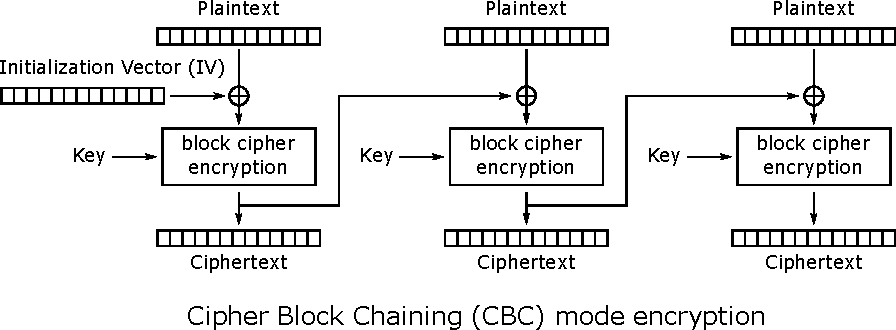
\includegraphics[width=\columnwidth]{CBC_encryption.pdf}
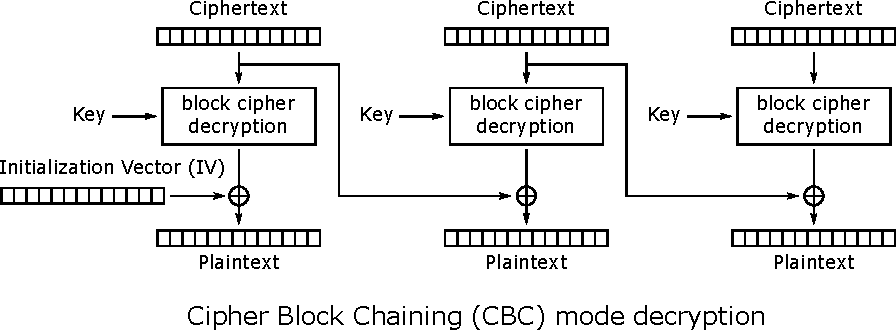
\includegraphics[width=\columnwidth]{CBC_decryption.pdf}
\(r=n, \quad c_0 = IV, \quad c_i = E_k(m_i \oplus c_i), \quad m_i = c_{i-1} \oplus E^{-1}_k (c-i)\), jeweils für $i\geq 1$\begin{itemize}[itemsep=1pt]
\item Bitfehler in \(c_i \Rightarrow m_i \) ist zufällig und  \(m_{i+1}\) hat den Bitfehler an gleicher Stelle wie \(c_i\), \(m_{i+2}\) und folgende werden dagegen wieder korrekt entschlüsselt.
\item Verlust von \(c_i \Rightarrow m_i \) ist verloren und  \(m_{i+1}\) ist zufällig (reparaturfähig), \(m_{i+2}\) und folgende werden dagegen wieder korrekt entschlüsselt.
\item Reparatur:  möglich durch $m_{i+1}^{korrigiert} = m_{i+1} \oplus m_i \oplus c_i$, nur durch Sender möglich.
\item Angriff: nicht möglich
\item Einsatz: Verschlüsselung von Dateien und langen Nachrichten, sehr beliebt
\end{itemize}

\subsubsection{CFB – Cipher Feedback}
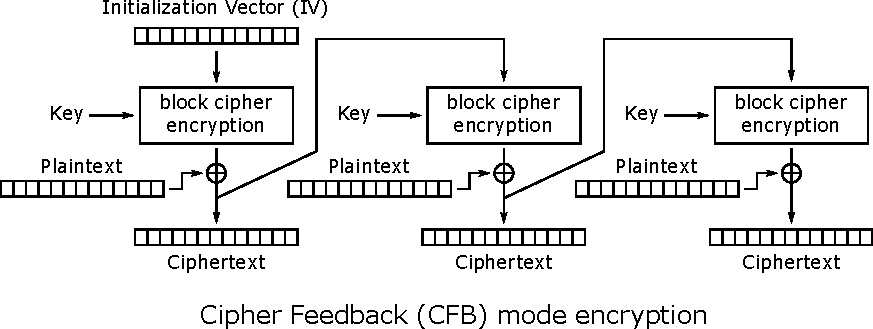
\includegraphics[width=\columnwidth]{CFB_encryption.pdf}
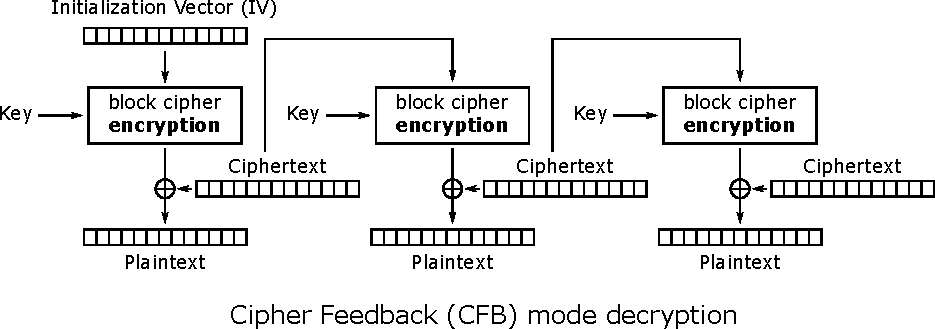
\includegraphics[width=\columnwidth]{CFB_decryption.pdf}
\(1 \leq r \leq n,~c_0 = \textrm{Initialvektor},~c_i = m_i \oplus msb_{r}(E_k(x_{i})),~m_i = c_i \oplus msb_{r}(E_k(x_{i})), \quad x_{i+1} = lsb_{n-r}(x_{i})~||~c_i\)
\begin{itemize}[itemsep=1pt]
\item Bitfehler in \(c_i \Rightarrow m_i \) mit Bitfehler an gleichen Stelle wie \(c_i\) und alle folgenden $\lceil\frac{n}{r}\rceil$ Blöcke sind zufällig. 
\item Verlust von \(c_i \Rightarrow m_i \) ist verloren, alle folgenden $\lceil\frac{n}{r}\rceil$ Blöcke sind zufällig. 
\item Reparatur: möglich durch $m_{i+1}^{korrigiert} = m_{i+1} \oplus E_k^{-1}(c_{i-1}) \oplus E_k^{-1}(c_{i}$
\item Angriff: nicht möglich
\item Einsatz: Stückweise anfallende, kleinere Datenmenge (Ströme)
\end{itemize}
\textbf{Entschlüsselungsverhalten für $r<n$}\\
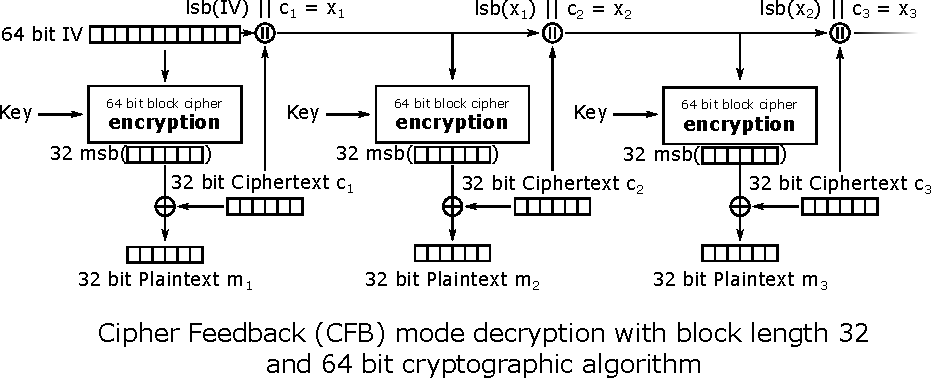
\includegraphics[width=\columnwidth]{CFB32_decryption.pdf}

\subsubsection{OFB – Output Feedback}
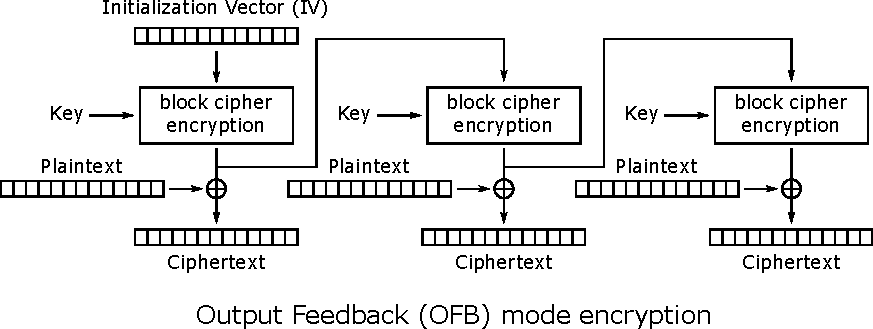
\includegraphics[width=\columnwidth]{OFB_encryption.pdf}
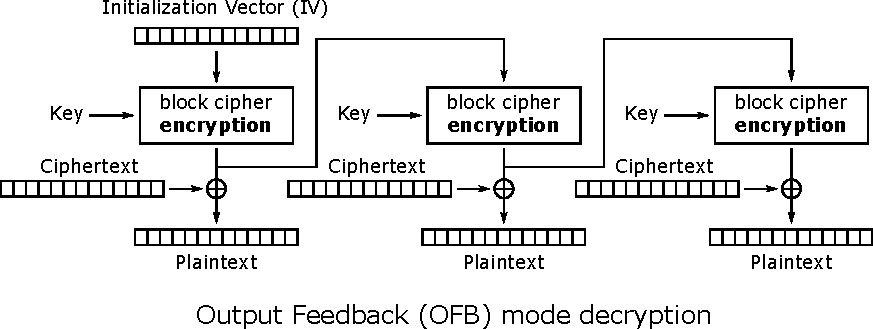
\includegraphics[width=\columnwidth]{OFB_decryption.pdf}
\(1 \leq r \leq n, \qquad V_0=\textrm{Initialvektor}, \qquad V_i=E_k(V_{i-1}), \qquad c_0 := V_0, \qquad c_i =msb_r(V_i) \oplus m_i, \qquad m_i =msb_r(V_i) \oplus c_i \) für \(1\leq i \leq n\).
\begin{itemize}[itemsep=1pt]
\item Bitfehler in \(c_i \Rightarrow m_i \) mit Bitfehler an der gleichen Stelle wie \(c_i\).
\item Verlust von \(c_i \Rightarrow m_i \) ist verloren, weitere Blöcke defekt (korrigierbar).
\item Reparatur: möglich
\item Angriff: bei gleichem Schlüssel und IV möglich.
\item Einsatz: Satellitenkommunikation (auf Grund der Fehlertoleranz), Filesysteme/Datenbanken wegen wahlfreiem Zugriff
\end{itemize}

\section{Kryptographische Hashfunktionen}
Eine Hashfunktion ist eine Funktion $h$, die mindestens folgende Eigenschaften erfüllt: \begin{itemize}
 \item \textbf{compression} $h$ bildet eine beliebig lange Nachricht $m$ auf einen Hashwert $h(m)$ mit der fixen Länge $n$ ab.
 \item \textbf{ease of computation} für gegebenes $h$ und $m$ muss es leicht sein, $h(m)$ zu berechnen.
 \end{itemize}

\subsection{MDC - Manipulation Detection Codes} MDCs (auch bekannt unter \textit{message integraty codes - MICs}) gehören zu der Obergruppe der \textit{unkeyed hash functions} und muss neben den oben genannten folgende Eigenschaften erfüllen:
\begin{itemize}
\item \textbf{Preimage Resistance:} Praktisch unmöglich, zu gegebenem Hashwert $H$ ein Dokument $m$ vorzuweisen mit $H = H(m)$
\item \textbf{Collision Resistance:} (auch \textit{stark kollisionsresistent} genannt) 
Praktisch unmöglich, zwei Dokumente $m \neq m'$ vorzuweisen mit $H(m) = H(m')$ 
\item \textbf{Second Preimage Resistance:} (auch \textit{schwach kollisionsresistent} genannt) Praktisch unmöglich, zu gegebenem Dokument $m$ ein zweites Dokument $m'$ vorzuweisen mit $m \neq m'$ und $H(m) = H(m')$ 
\end{itemize}

\begin{center}\textbf{Anmerkungen}\end{center}

\begin{itemize}
 \item[--] Eine \textit{starke kollisionsresistente} (collision-resistant) Hashfunktion ist auch \textit{schwach kollisionsrestistent} (second-pre-image resistant).
 \item[--] Eine \textit{schwach kollisionsrestistente} (second-pre-image resistant) Hashfunktion ist eine Einwegfunktion (one-way function).
 \item[--] Hashfunktionen sind durch die Voraussetzung der \textit{starken Kollisionsresistenz} (collision Restistance) mächtiger als Einwegfunktionen (one-way hash functions).
 \end{itemize}
 


\subsection{MAC - Message Authentication Codes}
Ein MAC-Algorithmus ist eine Funktion $h_k$, mit einem geheimen Schlüssel als Parameter $k$, die die folgenden Eigenschaften (neben den oben genannten erfüllt: \begin{itemize}
 \item \textbf{computation-resistance} Es ist schwer für Null oder mehr gegebene Nachrichten- MAC Paare $(m_i, h_k(m_i))$ ein Nachrichten-MAC Paar $(x, h_k(m))$ zu berechnen für das gilt $m \neq m_i$.
 \end{itemize}

\section{Kryptographische Protokolle}
\subsection{Diffie-Hellman-Schlüsselaustausch}
Alice und Bob haben einen gemeinsamen öffentlichen Schlüssel $(p,g)$, 
$p$ Primzahl, $g$ primitive Wurzel von $\mathbb{Z}_{p}$ (wenn $g$ keine primitive Wurzel ist, ist das Verfahren möglich aber unsicher).
\begin{enumerate}
    \item Alice wählt zufällig $a \in [0,p-2]$, rechnet 
          $c = g^a \bmod p$ und schickt $c$ an Bob
    \item Bob wählt zufällig $b \in [0,p-2]$, rechnet
          $d = g^b  \bmod p$ und schickt $d$ an Alice
    \item Alice rechnet $k = d^a \bmod p$
    \item Bob rechnet $k = c^b \bmod p$
\end{enumerate}

\paragraph{Signieren}
Alice signiert eine Nachricht $m$ mit dem Geheimschlüssel $d$. Signierte
Nachricht ist $(m, m^{d}) = (m, \sigma)$.
\paragraph{Verifizieren} Bob erhält $(m, \sigma)$ von Alice und nutzt ihr Public Key $e$.
Falls $m = \sigma^{e} = (m^{d})^{e}$, ok.

\paragraph{Mögliche Angriffe} Eve sendet Bob die \glqq Signatur\grqq\ $(m^{e}, m)$, Bob potenziert $m$ mit $e$ und ist reingefallen, da er $(m^{e}, m^{e})$ bekommt. \\
Oder sie schickt ihm eine schon gültige, aber quadrierte Signatur: $(m^2, \sigma^2)$.
\end{multicols}
\paragraph{Primzahlen}
\footnotesize 2,     3,     5,     7,    11,    13,    17,    19,    23,    29,    31,    37,    41,    43,
   47,    53,    59,    61,    67,    71,    73,    79,    83,    89,    97,   101,   103,   107,
  109,   113,   127,   131,   137,   139,   149,   151,   157,   163,   167,   173,   179,   181,
  191,   193,   197,   199,   211,   223,   227,   229,   233,   239,   241,   251,   257,   263,
  269,   271,   277,   281,   283,   293,   307,   311,   313,   317,   331,   337,   347,   349,
  353,   359,   367,   373,   379,   383,   389,   397,   401,   409,   419,   421,   431,   433,
  439,   443,   449,   457,   461,   463,   467,   479,   487,   491,   499,   503,   509,   521,
  523,   541,   547,   557,   563,   569,   571,   577,   587,   593,   599,   601,   607,   613,
  617,   619,   631,   641,   643,   647,   653,   659,   661,   673,   677,   683,   691,   701,
  709,   719,   727,   733,   739,   743,   751,   757,   761,   769,   773,   787,   797,   809,
  811,   821,   823,   827,   829,   839,   853,   857,   859,   863,   877,   881,   883,   887,
  907,   911,   919,   929,   937,   941,   947,   953,   967,   971,   977,   983,   991,   997,
 1009,  1013,  1019,  1021,  1031,  1033,  1039,  1049,  1051,  1061,  1063,  1069,  1087,  1091,
 1093,  1097,  1103,  1109,  1117,  1123,  1129,  1151,  1153,  1163,  1171,  1181,  1187,  1193,
 1201,  1213,  1217,  1223,  1229,  1231,  1237,  1249,  1259,  1277,  1279,  1283,  1289,  1291,
 1297,  1301,  1303,  1307,  1319,  1321,  1327,  1361,  1367,  1373,  1381,  1399,  1409,  1423,
 1427,  1429,  1433,  1439,  1447,  1451,  1453,  1459,  1471,  1481,  1483,  1487,  1489,  1493,
 1499,  1511,  1523,  1531,  1543,  1549,  1553,  1559,  1567,  1571,  1579,  1583,  1597,  1601,
 1607,  1609,  1613,  1619,  1621,  1627,  1637,  1657,  1663,  1667,  1669,  1693,  1697,  1699,
 1709,  1721,  1723,  1733,  1741,  1747,  1753,  1759,  1777,  1783,  1787,  1789,  1801,  1811,
 1823,  1831,  1847,  1861,  1867,  1871,  1873,  1877,  1879,  1889,  1901,  1907,  1913,  1931,
 1933,  1949,  1951,  1973,  1979,  1987,  1993,  1997,  1999,  2003,  2011,  2017,  2027,  2029,
 2039,  2053,  2063,  2069,  2081,  2083,  2087,  2089,  2099,  2111,  2113,  2129,  2131,  2137,
 2141,  2143,  2153,  2161,  2179,  2203,  2207
 Dez. zu Bin.: 1: 1, 2: 10, 3: 11, 4: 100, 5: 101, 6: 110, 7: 111, 8: 1000, 9: 1001, 10: 1010, 11: 1011, 12: 1100, 13: 1101, 14: 1110, 15: 1111, 16: 10000, 17: 10001, 18: 10010, 19: 10011, 20: 10100, 21: 10101, 22: 10110, 23: 10111
\end{document}
